\documentclass[10pt]{article}
\usepackage[a4paper,margin=2.2cm]{geometry}
\usepackage[T1]{fontenc}
\usepackage[utf8]{inputenc}
\usepackage{lmodern}
\usepackage{amsmath,amssymb,amsthm}
\usepackage{graphicx}
\usepackage{booktabs}
\usepackage{array}
\usepackage{caption}
\usepackage{microtype}
\usepackage[hidelinks]{hyperref}
\captionsetup{font=small,labelfont=bf,labelsep=period,justification=justified,singlelinecheck=false}
\graphicspath{{../figures/}}
\setlength{\parskip}{0.4em}
\setlength{\parindent}{0pt}
\newcommand{\Dh}{\hat D}
\newcommand{\ReP}{\mathrm{Re}\,\Phi_0}
\newcommand{\ImP}{\mathrm{Im}\,\Phi_0}
\newcommand{\sstart}{s_{\mathrm{start}}}
\renewcommand{\figurename}{Supplementary Fig.}
\renewcommand{\tablename}{Supplementary Table}
\newtheorem*{lemma}{Lemma}

\begin{document}
\begin{center}
{\Large\bfseries Supplementary Information\par}
\vspace{0.5em}
{\large A resonance phase locates unstable self-similar singularities beyond an exponential precision wall\par}
\vspace{0.4em}
{\small [Author names]\par}
\end{center}

\tableofcontents
\vspace{1em}

Every number in this document is generated from the logged outputs in \texttt{data/outputs} of the code and data
package: the tables are written by \path{code/analysis/make_si_tables.py} and the figures by
\path{code/figures/make_figures.py}. Evidence levels: [P] proved (elementary), [F] formal matched asymptotics,
[N] numerical with stated error.

%=====================================================================================================
\section*{Supplementary Note 1. Validation on 2D Boussinesq and the Hou--Luo model}
\addcontentsline{toc}{section}{Supplementary Note 1. Validation on 2D Boussinesq and the Hou--Luo model}

The pipeline used for IPM was first developed and validated on the 2D Boussinesq system with a boundary, the
standard proxy for axisymmetric Euler at a wall\cite{s_chen2022}, and on its one-dimensional boundary restriction,
the Hou--Luo model\cite{s_choi2017}. In both, $\varepsilon=\lambda-1$ in equation~(1) of the main text and the branch
is followed in $z=1/(\lambda-1)$.

\textbf{Profiles and two independent solvers (2D) [N].} The marching solver finds eight smooth profiles
$\lambda_0,\dots,\lambda_7$ (Supplementary Table~\ref{tab:bq}). The independent global solver (Methods), which shares
no numerical ingredient with it, reproduces all eight; with matched origin truncation the differences are at most
$4.6\times10^{-6}$. The deepest rungs are weakly determined ($|m-2|\lesssim10^{-6}$ nearby), the same exponential
wall as in IPM.

\begin{table}[h]
\centering
\caption{\textbf{2D Boussinesq profiles.} Marching solver ($h_s=0.0125$ from $n=4$); global solver extrapolated in
$s_{\max}$ (difference global $-$ marching). Source: \texttt{programs/P03\_boussinesq\_ladder} (\texttt{glob\_*},
\texttt{bq\_*} logs).}
\label{tab:bq}
\small
\begin{tabular}{rrrrr}
\toprule
$n$ & $\lambda_n$ & $z_n=1/(\lambda_n-1)$ & $z_n-z_{n-1}$ & global $-$ marching\\
\midrule
0 & 1.9205593 & 1.08630 & --- & $+1.7\times10^{-6}$\\
1 & 1.3990961 & 2.50566 & 1.41937 & $-1.1\times10^{-7}$\\
2 & 1.2523487 & 3.96277 & 1.45711 & $-5.6\times10^{-7}$\\
3 & 1.1842533 & 5.42733 & 1.46455 & $-3.2\times10^{-7}$\\
4 & 1.1449857 & 6.89723 & 1.46991 & $-4.2\times10^{-7}$\\
5 & 1.1194738 & 8.37004 & 1.47281 & $+1.1\times10^{-7}$\\
6 & 1.1015817 & 9.84429 & 1.47426 & $-4.6\times10^{-6}$ to $+0.4\times10^{-6}$\\
7 & 1.0883384 & 11.32010 & 1.47581 & $+2.1\times10^{-7}$ ($s_{\min}=-20$)\\
\bottomrule
\end{tabular}
\end{table}

\textbf{Instability index [N].} Perturbations grow as $e^{\mu\tau}$, $\tau=-\ln(1-t)$. Method~1 linearizes the march
and Biot--Savart map; $\mu$ is an eigenvalue if the linearized map $T_\mu$ has eigenvalue~1. Right-half-plane counts
by the argument principle applied to $\det(I-T_\mu)$, which include the trivial time-translation mode $\mu=1$, give
$1.997$, $3.000$, $4.000$, $5.000$, $5.952$, $6.942$ and $7.921$ zeros for the 2D profiles $n=1$--7: the $n$-th
profile has exactly $n$ unstable directions, all real, and the counts are unchanged under domain and grid variants.
Method~2, a shift-invert eigensolver on the global discretization, reproduces 27 of the 28 unstable eigenvalues of
$\lambda_1$--$\lambda_7$ to $5\times10^{-5}$; the remaining one lies in its truncation-artefact band and is confirmed
by method~1 with two truncations. In the Hou--Luo model (11 profiles) the index is $n$ for $n\le10$. In IPM, method~1
gives contour counts $0.994$, $1.947$, $3.082$, $4.077$ and $4.902$ for $n=0$--4 (\texttt{ipm\_contour\_U*.out}),
i.e.\ index $n$.

\textbf{Spacings [N].} For a stalled layer of fixed extent (2D Boussinesq, Hou--Luo) the spacings of $1/\varepsilon_n$
increase towards a constant; for IPM, whose layer recedes, they contract (Supplementary Fig.~\ref{fig:spacing}).

%=====================================================================================================
\section*{Supplementary Note 2. Error audit}
\addcontentsline{toc}{section}{Supplementary Note 2. Error audit}

\textbf{Front--grid locking.} Supplementary Table~\ref{tab:shift} lists $m-2$ on radial grids shifted by $\delta h_s$
around the seventh profile, and Supplementary Fig.~\ref{fig:shift} shows them. The scatter over shifts is the locking
error at that grid; its half-range falls from $\sim10^{-6}$ ($h_s=0.025$) to $\sim10^{-8}$ ($0.0125$) and
$\sim10^{-10}$ ($0.00625$), i.e.\ as $h_s^{7.1}$ (main-text Fig.~3a). On $h_s=0.025$ the scatter exceeds the defect
itself, which is why that grid produced a spurious zero near $z=6.905$ (pre-registration record, stage 2d).

\begin{figure}[h]
\centering
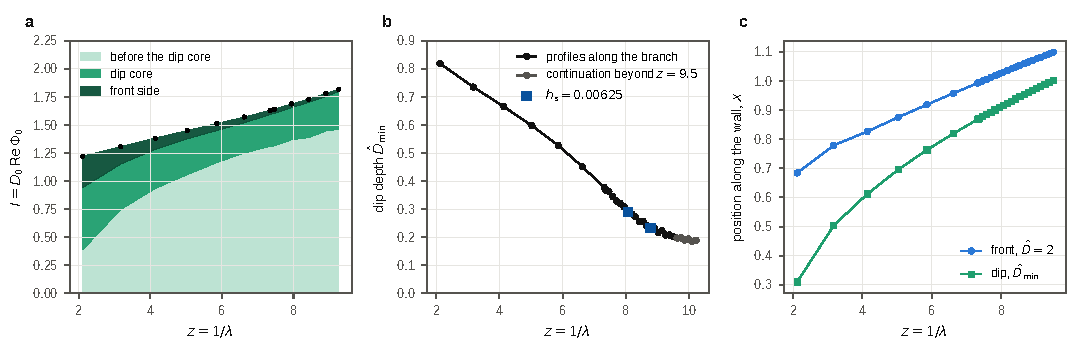
\includegraphics[width=\textwidth]{SupplementaryFig1.pdf}
\caption{\textbf{Raw grid-shift data near the seventh profile.} $m-2$ on four radial grids shifted by
$\delta h_s$ ($\delta=0,\tfrac14,\tfrac12,\tfrac34$; symbols offset slightly in $z$ by $\delta$) and their mean (line),
for $h_s=0.025$ (\textbf{a}), $0.0125$ (\textbf{b}) and $0.00625$ (\textbf{c}). Only on the finest grid does the scatter
fall below the defect.}
\label{fig:shift}
\end{figure}

\begin{table}[h]
\centering
\caption{\textbf{Grid-shift data} (\texttt{rich7\_*.out}; unshifted values from the scans \texttt{ipm\_scan\_\{p7,h7\}}).}
\label{tab:shift}
\small
\begin{tabular}{rrrrrrr}
\toprule
$z$ & $h_s$ & $\delta=0$ & $\delta=\tfrac14$ & $\delta=\tfrac12$ & $\delta=\tfrac34$ & half-range\\
\midrule
7.256 & 0.00625 & $4.85\times10^{-9}$ & $4.93\times10^{-9}$ & $4.84\times10^{-9}$ & $4.96\times10^{-9}$ & $6.0\times10^{-11}$\\
7.256 & 0.025 & $5.21\times10^{-7}$ & $-1.35\times10^{-6}$ & $2.46\times10^{-6}$ & $2.11\times10^{-6}$ & $1.9\times10^{-6}$\\
7.316 & 0.00625 & $1.00\times10^{-9}$ & $8.80\times10^{-10}$ & $9.40\times10^{-10}$ & $8.20\times10^{-10}$ & $9.1\times10^{-11}$\\
7.316 & 0.0125 & $1.14\times10^{-8}$ & $1.47\times10^{-8}$ & $-7.22\times10^{-9}$ & $2.45\times10^{-9}$ & $1.1\times10^{-8}$\\
7.316 & 0.025 & $1.94\times10^{-6}$ & $-6.79\times10^{-8}$ & $2.05\times10^{-6}$ & $2.82\times10^{-6}$ & $1.4\times10^{-6}$\\
7.346 & 0.00625 & $3.01\times10^{-11}$ & $-6.21\times10^{-11}$ & $5.56\times10^{-11}$ & $-1.16\times10^{-10}$ & $8.6\times10^{-11}$\\
7.376 & 0.00625 & $-7.35\times10^{-10}$ & $-7.21\times10^{-10}$ & $-7.65\times10^{-10}$ & $-6.46\times10^{-10}$ & $6.0\times10^{-11}$\\
7.376 & 0.0125 & $-3.92\times10^{-9}$ & $8.43\times10^{-9}$ & $-1.61\times10^{-8}$ & $-1.40\times10^{-8}$ & $1.2\times10^{-8}$\\
7.376 & 0.025 & $3.05\times10^{-6}$ & $1.58\times10^{-6}$ & $8.27\times10^{-7}$ & $2.72\times10^{-6}$ & $1.1\times10^{-6}$\\
\bottomrule
\end{tabular}

\smallskip\par\footnotesize $m-2$ on radial grids shifted by $\delta h_s$ ($s_{\min}\to-120+\delta h_s$).

\end{table}

\textbf{Origin truncation and the Newton floor.} Supplementary Table~\ref{tab:trunc} gives the converged Newton
residual and $m-2$ for origin truncations $\sstart=-15$ to $-30$ at $\lambda_5$ and $\lambda_6$. The offset relative to
$\sstart=-20$ decays roughly as $e^{\sstart}$ down to $-19$ (the neglected local corrections are $O(e^{\sstart})$);
deeper starts raise the residual floor and add a round-off offset that is independent of $\lambda$ at $-24$
($1.5\times10^{-9}$ at both $\lambda_5$ and $\lambda_7$) and reaches $2.1\times10^{-8}$ at $-30$.

\begin{table}[h]
\centering
\caption{\textbf{Origin truncation and Newton residual floor.}}
\label{tab:trunc}
\small
\begin{tabular}{rrrr}
\toprule
profile & $s_{\rm start}$ & Newton residual $|R|$ & $m-2$\\
\midrule
$\lambda_5$ & -16 & $1.1\times10^{-13}$ & $-5.12\times10^{-9}$\\
$\lambda_5$ & -20 & $5.2\times10^{-13}$ & $2.32\times10^{-11}$\\
$\lambda_5$ & -24 & $7.9\times10^{-13}$ & $-1.48\times10^{-9}$\\
$\lambda_6$ & -15 & $7.3\times10^{-13}$ & $2.16\times10^{-8}$\\
$\lambda_6$ & -16 & $3.6\times10^{-14}$ & $-4.92\times10^{-9}$\\
$\lambda_6$ & -17 & $1.5\times10^{-13}$ & $-8.95\times10^{-10}$\\
$\lambda_6$ & -18 & $2.0\times10^{-13}$ & $1.43\times10^{-9}$\\
$\lambda_6$ & -19 & $4.8\times10^{-13}$ & $7.92\times10^{-10}$\\
$\lambda_6$ & -20 & $4.4\times10^{-13}$ & $5.76\times10^{-10}$\\
$\lambda_6$ & -26 & $1.9\times10^{-12}$ & $8.28\times10^{-9}$\\
$\lambda_6$ & -30 & $1.5\times10^{-11}$ & $2.19\times10^{-8}$\\
\bottomrule
\end{tabular}

\smallskip\par\footnotesize $h_s=0.0125$, $N_b=32$; $\lambda_6=0.15092$, $\lambda_5=0.1706180880$.

\end{table}

\textbf{Angular resolution at the sixth profile.} With $\sstart=-16$, $N_b=32\to48$ changes $m$ by $2.0\times10^{-8}$
and $N_b=48\to64$ by $9\times10^{-11}$ (\texttt{ipm\_nbcheck*\_lam6.out}); with $\sstart=-20$ the $N_b=32\to48$ change
is $\sim10^{-9}$ for $\lambda_4$--$\lambda_6$. At the seventh profile $N_b=48\to64$ changes $m$ by $2.3\times10^{-9}$
(Extended Data Table~1 of the main text): the angular error stops converging at the floor. Tightening the Newton tolerance from $10^{-11}$
to $10^{-13}$ changes $m$ by $1.7\times10^{-11}$ (\texttt{ipm\_noise\_lam6\_hs0125.out}), so the scatter at the floor
is discretization, not the nonlinear solver.

\textbf{Two independent solvers (IPM).} Supplementary Table~\ref{tab:two} compares the independent global solver
with the marching solver. Converted with the crossing slopes, the differences are $0.2$--$3.5\times10^{-9}$ in $m$ at
every profile, while the difference in profile position grows by five orders of magnitude.

\begin{table}[h]
\centering
\caption{\textbf{IPM profiles from two independent solvers} (\texttt{ipm\_glob\_*.log}). At $h_s=0.00625$ the global
solver did not converge for $n=5$, $6$ within 15 Newton iterations (logged, not used).}
\label{tab:two}
\small
\begin{tabular}{rrrrrr}
\toprule
$n$ & $\lambda_n$ (marching) & $|\Delta\lambda|$ & $|\Delta z|$ & $|dm/d\lambda|$ & $|\Delta m|$\\
\midrule
1 & 0.4721297348 & $1.4\times10^{-8}$ & $6.4\times10^{-8}$ & $2.4\times10^{-1}$ & $3.5\times10^{-9}$\\
2 & 0.3149618108 & $3.7\times10^{-8}$ & $3.8\times10^{-7}$ & $6.0\times10^{-2}$ & $2.2\times10^{-9}$\\
3 & 0.2415663353 & $3.4\times10^{-8}$ & $5.9\times10^{-7}$ & $1.1\times10^{-2}$ & $3.8\times10^{-10}$\\
4 & 0.1987224523 & $6.5\times10^{-7}$ & $1.7\times10^{-5}$ & $1.7\times10^{-3}$ & $1.1\times10^{-9}$\\
5 & 0.1706180880 & $9.1\times10^{-7}$ & $3.1\times10^{-5}$ & $2.3\times10^{-4}$ & $2.1\times10^{-10}$\\
6 & 0.1509200000 & $1.3\times10^{-4}$ & $5.9\times10^{-3}$ & $2.0\times10^{-5}$ & $2.7\times10^{-9}$\\
\bottomrule
\end{tabular}

\smallskip\par\footnotesize Independent global solver ($h_s=0.0125$, $s_{\min}=-16$, extrapolated in $s_{\max}$; $n=1$ at $h_s=0.025$, $s_{\min}=-12$; $n=4$ at $h_s=0.00625$) against the marching solver. $|\Delta m|=|dm/d\lambda|\,|\Delta\lambda|$.

\end{table}

%=====================================================================================================
\section*{Supplementary Note 3. The pre-registration record}
\addcontentsline{toc}{section}{Supplementary Note 3. The pre-registration record}

All predictions for IPM were committed to the public repository before the computation they concern, in
\texttt{programs/P03\_boussinesq\_ladder/PREDICTIONS\_IPM.md}; entries are never edited, and outcomes, deviations
and corrections are appended. The time stamps are those of the commits that touch the file
(\texttt{git log} on the file); a copy of the record as of submission is provided as Supplementary Data~1.

\begin{table}[h]
\centering
\caption{\textbf{Timeline of the record.}}
\small
\begin{tabular}{>{\raggedright\arraybackslash}p{2.3cm}>{\raggedright\arraybackslash}p{6.2cm}>{\raggedright\arraybackslash}p{6.4cm}}
\toprule
Commit & Registered & Outcome (appended later)\\
\midrule
\texttt{4dc82af} & Stage 1, before any IPM continuation: accumulation as $\lambda\to0$, linear law, index $n$, lattice
of growth rates of step $\lambda_n$, rigid spectral flow, localization at the front & Accumulation clause and linear
law failed (spacings contract by 0.92 per profile); index $n$ ($n=0$--4), lattice, flow and localization held\\
stage 2 entries & $\lambda_3$, $\lambda_4$, $\lambda_5$, $\lambda_6$ and the growth rates of the fourth unstable profile
from the lower profiles by fixed rules & Errors 6\%, 2.5\%, 2\%, 0.1\% of a spacing; growth rates to 0.2--1.2\%\\
\texttt{c922751} & Stage 3: $z_7$, $z_8$ by three rung-fit rules (H1, H1$'$, H2, H3) & $z_7$: not decisive (main
text); $z_8$: untested\\
\texttt{273ae28} & Stage 3, H4: $z_7=7.352$, $z_8\approx7.91$--$7.92$ (low confidence) from the phase on the coarse
branch & $z_7$: not decisive; the $z_8$ value was made with the faulty tracker (Supplementary Note~5)\\
\texttt{f0b3f06} & Decision rule for $\lambda_7$, fixed before the crossing was known & Could not run as written (scan
paused); converged-grid analysis reported with the same thresholds\\
\texttt{251bf1e} & Stage 4: $\lambda_8$--$\lambda_{10}$ from the repaired phase, with bands, required precision and a
decision rule & Open benchmark (Supplementary Table~\ref{tab:stage4})\\
\bottomrule
\end{tabular}
\end{table}

\textbf{Deviations and corrections recorded in the file.} (i) The committed $\lambda_7$ procedure needed matched scans
at $h_s=0.0125$ and $0.00625$; the $0.0125$ scan had been paused to measure the locking error, so the procedure could
not complete; the converged-grid determination with four grid shifts was reported instead, judged by the same
thresholds. (ii) A first phase reading of $\lambda_7$ ($z_7=7.3456\pm0.003$) was corrected the same day to
$7.341\pm0.005$ (dependence on the offset) and, after the tracker repair, to $7.354\pm0.007$; none of these is a
registered prediction. (iii) The tracker failure and its repair were recorded with a clarification that the failure
counter had been logged but not gated.

\textbf{Stage 4.} The rule: solve $\ReP(z_n)=n\pi+\delta_n$ with $\ReP$ from the repaired deep table (smoothed by a
local quadratic over $\pm0.5$ in $z$, shifted by the measured grid correction $+0.027\pm0.010$); offset scenarios
$\delta=\delta_6=1.974$ (central), $\delta=2.031$ (mean of $n=1$--5), and a continuing drift
$\delta_n=1.974-0.057(n-6)$; band = scenarios widened by the grid spread and the fit error. The required precision
continues the $\lambda_7$ crossing slope with the decay per half-period predicted by $\ImP$ times $(1+\lambda)$. A future
measurement counts only if $\sigma_z\le0.01$; it confirms the rule at $n$ if the measured $z_n$ lies inside the band
(widened by $2\sigma_z$), and refutes it otherwise. All values of $m-2$ computed in this range before registration were
at or below the floor and are disclosed in the record.

\begin{table}[h]
\centering
\caption{\textbf{Stage-4 predictions and the precision a test needs} (\texttt{ipm\_stage4\_predictions.out}).}
\label{tab:stage4}
\footnotesize
\setlength{\tabcolsep}{3pt}
\begin{tabular}{rrcrcrrrr}
\toprule
$n$ & $z_n$ & band & $\lambda_n$ & $\lambda$ band & e-folds/profile & $|dm/dz|$ & $\sigma_m$ ($\sigma_z=0.01$) & $\sigma_m$ ($\sigma_z=0.003$)\\
\midrule
8 & 7.9994 & [7.9700, 8.0172] & 0.125010 & [0.124732, 0.125471] & 2.74 & $1.8\times10^{-9}$ & $1.8\times10^{-11}$ & $5.3\times10^{-12}$\\
9 & 8.6282 & [8.5895, 8.6450] & 0.115899 & [0.115673, 0.116421] & 2.77 & $1.2\times10^{-10}$ & $1.2\times10^{-12}$ & $3.6\times10^{-13}$\\
10 & 9.2013 & [9.1575, 9.2142] & 0.108680 & [0.108528, 0.109200] & 3.06 & $5.9\times10^{-12}$ & $6.0\times10^{-14}$ & $1.8\times10^{-14}$\\
\bottomrule
\end{tabular}

\end{table}

%=====================================================================================================
\section*{Supplementary Note 4. The resonance phase}
\addcontentsline{toc}{section}{Supplementary Note 4. The resonance phase}

\textbf{Why a defect of this form has zeros [P].}
\begin{lemma}
Let $F(z)=R(z)\,[\cos\Theta(z)+\eta(z)]$ on $[z_0,\infty)$ with $R>0$ and $\Theta$ continuous, $\Theta$ strictly
increasing to $\infty$, and $\sup|\eta|<1$. Then $F$ changes sign between $\Theta^{-1}(k\pi)$ and $\Theta^{-1}((k+1)\pi)$
for every admissible integer $k$, so it has infinitely many zeros accumulating only at $z=\infty$; if $\eta\to0$, each
zero $z^*$ satisfies $\Theta(z^*)=(k+\tfrac12)\pi+O(|\eta(z^*)|)$.
\end{lemma}
\textit{Proof.} $F(\Theta^{-1}(k\pi))=R\,[(-1)^k+\eta]$ has the sign of $(-1)^k$ because $|\eta|<1$; apply the
intermediate value theorem. The second statement follows from $\cos\Theta=-\eta$. $\square$

\textbf{The stalled layer and the local problem [F].} As $\varepsilon\to0$ the wall speed $D=V_1/x$ is $O(\varepsilon)$
between the stagnation point and a front. In this layer we write a perturbation of the density as
$\tilde r(Y)\,e^{i\varphi}$ with $\varphi=D_0^{-1}\int\kappa\,ds$, $s=\ln x$, and $Y$ the wall-normal coordinate scaled
with the layer thickness, and keep the leading order in $\varepsilon$. For IPM this gives the local eigenproblem of
the Methods,
\begin{equation*}
\bigl[i\kappa(\Dh+\hat cY)+\mu Y\partial_Y\bigr]\tilde r=-G\,\partial_Y\tilde\psi+i\kappa R_y\tilde\psi ,\qquad
-\partial_Y^2\tilde\psi+\kappa^2\tilde\psi=-i\kappa\tilde r ,
\end{equation*}
with $\tilde\psi(0)=0$, no growing mode, $\Dh=D/D_0$, $\hat c=G=\partial_xR$ at the wall (because $\Omega=-\partial_1R$),
$\mu$ the wall-normal strain and $R_y$ the normal density gradient. The continued root $\kappa(s)$ defines the phase
$\Phi_0=D_0^{-1}\int\kappa\,ds$, integrated from the stagnation point to the front. Matching the layer solution to the
stagnation-point region and to the front writes the smoothness defect as
$m-2\simeq|A|\,e^{-|\ImP|}\,[\cos(\ReP+\arg A)+\eta]$ with $\eta=O(\varepsilon)$, so by the Lemma the smooth profiles
satisfy $\ReP(\lambda_n)=n\pi+\delta$ (main-text equation~(2)), and the envelope of the defect decays by
$e^{-|\Delta\ImP|}$ per half-period. The offset $\delta$ collects the $O(1)$ connection phases at the stagnation point
and at the front and is fixed by the cut-off convention $D/D_0=2$. The derivation is formal; its hypotheses are checked
numerically below.

\textbf{Exact scaling in IPM [P].} Substitute $Y=\Dh\,\eta$, $\kappa=K/\Dh$ and $\tilde r=\hat r/\Dh$. Then
$i\kappa(\Dh+\hat cY)=iK(1+\hat c\,\eta)$, $\mu Y\partial_Y=\mu\eta\partial_\eta$ and $\partial_Y=\Dh^{-1}\partial_\eta$,
and both equations become independent of $\Dh$:
\begin{equation*}
\bigl[iK(1+\hat c\eta)+\mu\eta\partial_\eta\bigr]\hat r=-G\,\partial_\eta\tilde\psi+iKR_y\tilde\psi ,\qquad
-\partial_\eta^2\tilde\psi+K^2\tilde\psi=-iK\hat r .
\end{equation*}
Hence $\kappa=K(G,\mu,R_y)/\Dh$ exactly and $\Phi_0=\int K\,ds/D$. Numerically $K$ is unchanged to $10^{-7}$ when
$\Dh$ is varied from $0.012$ to $2$ at fixed $(G,\mu,R_y)$ (main-text Fig.~5d; \texttt{ipm\_K\_checks.out}). In 2D
Boussinesq the vorticity obeys its own transport equation, which breaks this scaling.

\textbf{The phase along the branch [N].} Supplementary Table~\ref{tab:phase} lists the repaired phase on every
computed state. The offsets $\delta_n$ for four cut-offs are in Supplementary Table~\ref{tab:cut}: the registered
cut-off $D/D_0=2$ is the only one that is flat over $n=1$--5, and every cut-off shows an extra drop of
$0.04\pm0.01$ at $n=6$, which therefore originates inside the layer. Supplementary Table~\ref{tab:decay} compares the
decay of the defect per half-period with the prediction from $\ImP$.

\begin{table}[h]
\centering
\caption{\textbf{Offsets $\delta_n$ for four front cut-offs} (\texttt{ipm\_cutoff\_drift.out}).}
\label{tab:cut}
\small
\begin{tabular}{rrrrr}
\toprule
$n$ & cut-off 1.5 & cut-off 2 & cut-off 3 & cut-off 5\\
\midrule
1 & 1.7506 & 2.0331 & 2.3488 & 2.6849\\
2 & 1.7927 & 2.0228 & 2.2863 & 2.5643\\
3 & 1.8325 & 2.0320 & 2.2660 & 2.5144\\
4 & 1.8604 & 2.0360 & 2.2476 & 2.4712\\
5 & 1.8731 & 2.0301 & 2.2200 & 2.4232\\
6 & 1.8500 & 1.9742 & 2.1562 & 2.3253\\
\bottomrule
\end{tabular}

\smallskip\par\footnotesize Offsets $\delta_n=\mathrm{Re}\,\Phi_0(\lambda_n)-n\pi$ with the repaired tracker for four front cut-offs $D/D_0$; no untracked points. Cut-off 2 is the registered convention.

\end{table}

\begin{table}[h]
\centering
\caption{\textbf{Decay of the defect per half-period: prediction from $\ImP$ and measurement.}}
\label{tab:decay}
\small
\begin{tabular}{rrrrr}
\toprule
$z$ (midpoint) & $\lambda$ & predicted & measured & (meas.$-$pred.)/(pred.$\,\lambda$)\\
\midrule
2.96 & 0.338 & 1.73 & 2.30 & 0.97\\
3.96 & 0.253 & 1.85 & 2.32 & 1.02\\
4.88 & 0.205 & 1.95 & 2.37 & 1.04\\
5.68 & 0.176 & 2.05 & 2.56 & 1.42\\
6.45 & 0.155 & 2.14 & 2.38 & 0.70\\
\bottomrule
\end{tabular}

\smallskip\par\footnotesize E-folds of the defect per half-period: predicted $-\pi\,d\,\mathrm{Im}\Phi_0/d\,\mathrm{Re}\Phi_0$ from the repaired phase; measured from consecutive extrema of $|m-2|$.

\end{table}

\begin{table}[p]
\centering
\captionsetup{justification=raggedright}
\caption{\textbf{Repaired resonance phase on every computed state} (\texttt{ipm\_phase3\_\{rungs,l7,deep\}.out}).}
\label{tab:phase}
\footnotesize
\begin{tabular}{rrrrrrrl}
\toprule
$z$ & $D_0$ & $\hat D_{\rm dip}$ & $s_{\rm cut}$ & $\mathrm{Re}\,\Phi_0$ & $\mathrm{Im}\,\Phi_0$ & $I$ & untracked\\
\midrule
2.1181 & 0.23606 & 0.8194 & -0.380 & 5.1747 & -1.9087 & 1.22156 & 0\\
3.1750 & 0.15748 & 0.7353 & -0.250 & 8.3059 & -3.5978 & 1.30803 & 0\\
4.1396 & 0.12078 & 0.6657 & -0.191 & 11.4568 & -5.4154 & 1.38378 & 0\\
5.0321 & 0.09936 & 0.5971 & -0.133 & 14.6024 & -7.3379 & 1.45091 & 0\\
5.8610 & 0.08531 & 0.5276 & -0.085 & 17.7381 & -9.3555 & 1.51322 & 0\\
6.6260 & 0.07546 & 0.4515 & -0.043 & 20.8238 & -11.4252 & 1.57136 & 0\\
7.3160 & 0.06834 & 0.3750 & -0.007 & 23.8203 & -13.5550 & 1.62796 & 0\\
7.3460 & 0.06806 & 0.3717 & -0.006 & 23.9580 & -13.6584 & 1.63068 & 0\\
7.3760 & 0.06779 & 0.3674 & -0.004 & 24.0928 & -13.7557 & 1.63319 & 0\\
7.4660 & 0.06697 & 0.3636 & +0.000 & 24.5106 & -14.0662 & 1.64148 & 0\\
7.5860 & 0.06591 & 0.3458 & +0.006 & 25.0602 & -14.4663 & 1.65174 & 0\\
7.7060 & 0.06488 & 0.3293 & +0.012 & 25.6446 & -14.9372 & 1.66393 & 0\\
7.8260 & 0.06389 & 0.3204 & +0.018 & 26.2192 & -15.3738 & 1.67514 & 0\\
7.9460 & 0.06292 & 0.3083 & +0.024 & 26.8226 & -15.8768 & 1.68781 & 0\\
8.0660 & 0.06199 & 0.2902 & +0.030 & 27.4185 & -16.3487 & 1.69964 & 0\\
8.1860 & 0.06108 & 0.2834 & +0.035 & 27.9493 & -16.7308 & 1.70714 & 0\\
8.3060 & 0.06020 & 0.2729 & +0.041 & 28.6510 & -17.3721 & 1.72472 & 0\\
8.4260 & 0.05934 & 0.2565 & +0.047 & 29.1547 & -17.6826 & 1.73005 & 0\\
8.5460 & 0.05851 & 0.2570 & +0.052 & 29.7744 & -18.1999 & 1.74201 & 0\\
8.6660 & 0.05770 & 0.2413 & +0.058 & 30.4093 & -18.7190 & 1.75452 & 0\\
8.7860 & 0.05691 & 0.2322 & +0.063 & 31.0771 & -19.3427 & 1.76856 & 0\\
8.9060 & 0.05614 & 0.2339 & +0.068 & 31.7197 & -19.8606 & 1.78080 & 0\\
9.0260 & 0.05540 & 0.2170 & +0.073 & 32.3954 & -20.5066 & 1.79456 & 0\\
9.1460 & 0.05467 & 0.2238 & +0.079 & 33.0543 & -21.0476 & 1.80703 & 0\\
9.2660 & 0.05396 & 0.2080 & +0.084 & 33.7243 & -21.6692 & 1.81979 & 0\\
9.3860 & 0.05327 & 0.2081 & +0.089 & 34.6567 & -22.5874 & 1.84619 & 11 (excluded)\\
\bottomrule
\end{tabular}

\smallskip\par\footnotesize Rungs $n=1$--5 and $\lambda_6$ on $h_s=0.0125$; $z=7.316$--$7.376$ on $h_s=0.00625$; deep states on $h_s=0.0125$ (continuation). $I=D_0\,\mathrm{Re}\,\Phi_0$.

\end{table}

%=====================================================================================================
\section*{Supplementary Note 5. The tracker failure and its repair}
\addcontentsline{toc}{section}{Supplementary Note 5. The tracker failure and its repair}

\textbf{Original tracker.} Along the wall, the root $\kappa$ at the next point was sought from the previous $\kappa$
(and from the Hou--Luo closed form as a fallback); a point without an accepted root kept the previous $\kappa$ and was
counted as failed. On the shallow states no point failed.

\textbf{Failure.} On the deep states the front side of the dip carries $\Dh$ from about $0.3$ to $2$ within a few steps
of $\Delta s=0.025$. The previous $\kappa$ is then a poor predictor, the secant iteration lands on another root or
fails, and holding $\kappa$ inflates $K=\kappa\Dh$ in proportion to $\Dh$. Supplementary Table~\ref{tab:tracker}
compares $I=D_0\ReP$ from the original and the repaired tracker; the original values are non-monotone in $z$ and
exceed the repaired ones by up to 14\%.

\textbf{Repair.} Up to the dip the original tracking is kept. Beyond it: (i) step $\Delta s/4$; (ii) predictor
$K_{\rm prev}/\Dh$ (exact by the scaling of Supplementary Note~4), then the previous $\kappa$, then the Hou--Luo form;
(iii) accept a root only if $|K-K_{\rm prev}|\le0.25|K_{\rm prev}|$; (iv) at a failed point hold $K$, not $\kappa$, and
count it; (v) exclude any state with a failed point from every fit. The repaired tracker reproduces the shallow values
($\ReP=11.4568$ vs $11.4566$ at $n=3$; $17.7381$ vs $17.7363$ at $n=5$) and fails on one of 17 deep states
($z=9.386$, 11 points; excluded).

\begin{table}[h]
\centering
\captionsetup{justification=raggedright}
\caption{\textbf{Phase coefficient from the original and the repaired tracker} (\texttt{ipm\_wkb\_e5\_cut2.out},
\texttt{ipm\_tracker\_diag.out}).}
\label{tab:tracker}
\small
\begin{tabular}{rrrr}
\toprule
$z$ & $I$, original tracker & failed points (counted) & $I$, repaired tracker\\
\midrule
6.626 & 1.57134 & 0 & 1.57136\\
6.746 & 1.58478 & 0 & --\\
6.866 & 1.59341 & 0 & --\\
7.466 & 1.64395 & 0 & 1.64148\\
7.586 & 1.65870 & 2 & 1.65174\\
7.706 & 1.72326 & 3 & 1.66393\\
7.826 & 1.74614 & 3 & 1.67514\\
7.946 & 1.92056 & 4 & 1.68781\\
8.066 & 1.74702 & 3 & 1.69964\\
8.186 & 1.85564 & 4 & 1.70714\\
8.306 & 1.88404 & 4 & 1.72472\\
8.426 & 1.91985 & 4 & 1.73005\\
8.546 & 1.95728 & 4 & 1.74201\\
8.666 & 1.98989 & 4 & 1.75452\\
\bottomrule
\end{tabular}

\end{table}

%=====================================================================================================
\section*{Supplementary Note 6. The deep branch and the endpoint analysis}
\addcontentsline{toc}{section}{Supplementary Note 6. The deep branch and the endpoint analysis}

\textbf{Geometry [N].} Supplementary Table~\ref{tab:geom} and Supplementary Fig.~\ref{fig:deep} give the dip depth,
the dip and front positions, the travel time $T=\int ds/\Dh$, the steepest wall gradient and the resolution indicator
along the branch. Supplementary Table~\ref{tab:deepres} compares two deep states on $h_s=0.0125$ and $0.00625$: the
geometry and $T$ agree to 0.3\%, while the indicator, the steepest gradient and $m-2$ change as described in the main
text.

\begin{figure}[h]
\centering
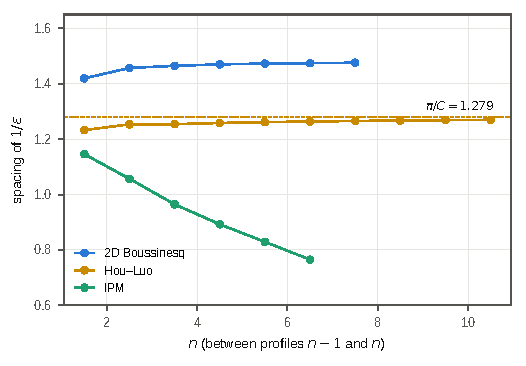
\includegraphics[width=\textwidth]{SupplementaryFig2.pdf}
\caption{\textbf{Geometry of the IPM branch.} \textbf{a}, Partition of $I=D_0\ReP$: the part before the dip core
(inner layer and approach) grows as the dip and front recede; the dip core and the front side do not. \textbf{b}, Dip
depth $\Dh_{\min}$ along the branch, with two checks at $h_s=0.00625$. \textbf{c}, Positions of the dip and of the
front ($\Dh=2$).}
\label{fig:deep}
\end{figure}

\begin{figure}[h]
\centering
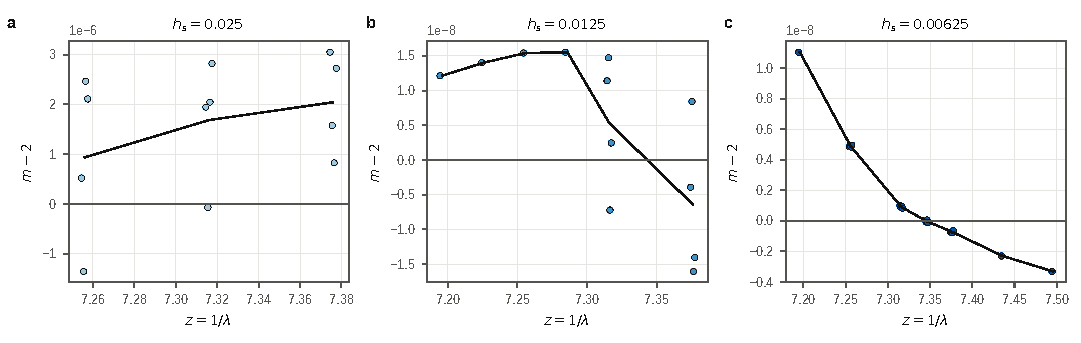
\includegraphics[width=0.5\textwidth]{SupplementaryFig3.pdf}
\caption{\textbf{Spacings of consecutive profiles in $1/\varepsilon$.} A stalled layer of fixed extent gives
increasing spacings (2D Boussinesq, Hou--Luo; dashed: the Hou--Luo asymptote $\pi/C=1.279$ obtained from the
$\lambda\to1$ limit problem); the receding layer of IPM gives contracting spacings.}
\label{fig:spacing}
\end{figure}

\textbf{Endpoint classes [N].} The phase coefficient $I(z)$ was fitted on $z\ge4$ with three forms: (A)
$a+bz+cz^2$ (accumulation at $\lambda=0$); (B) $a+bz+C/(z_c-z)$ and (C) $a+bz-C\ln(1-z/z_c)$ (accumulation at
$\lambda_c=1/z_c$). Weighting the shallow points by their grid error and the deep points by their scatter, (B) and (C)
prefer $z_c\approx10$--$13$ with $\chi^2\approx33$--$36$ for 20 degrees of freedom, against $\chi^2=140$ for (A); the
fits are therefore not adequate models and the preference is not significant. On the deep range alone ($z\ge7.45$),
$z_c$ is unconstrained ($\Delta\chi^2\le4$ for all $z_c\ge9.5$), the slope of $I$ is $0.098$ and its curvature
$+0.005\pm0.002$. Termination indicators: $\Dh_{\min}$ and $1/\max\partial_xR$ decrease at $-0.107$ and $-0.050$ per
unit $z$ on $z\in[7.45,8.5]$ and at $-0.023$ and $-0.014$ over the last unit, extrapolating linearly to zero only near
$z\approx18$ and $13$ (\texttt{ipm\_endpoint\_geometry.out}). The endpoint class is unresolved.

\begin{table}[p]
\centering
\caption{\textbf{Geometry along the IPM branch} (\texttt{ipm\_travel\_time.out}, \texttt{ipm\_deep\_e5.out}).}
\label{tab:geom}
\footnotesize
\begin{tabular}{rrrrrrr}
\toprule
$z$ & $\hat D_{\min}$ & $x_{\rm dip}$ & $x_{\rm cut}$ & $T$ & max $\partial_xR$ & indicator (\%)\\
\midrule
2.118 & 0.8194 & 0.3098 & 0.6841 & 9.6691 & -- & --\\
3.175 & 0.7353 & 0.5040 & 0.7790 & 9.8360 & -- & --\\
4.140 & 0.6657 & 0.6117 & 0.8265 & 9.9403 & -- & --\\
5.032 & 0.5971 & 0.6956 & 0.8753 & 10.0315 & -- & --\\
5.861 & 0.5276 & 0.7633 & 0.9186 & 10.1126 & -- & --\\
6.626 & 0.4515 & 0.8195 & 0.9577 & 10.1880 & -- & --\\
7.316 & 0.3781 & 0.8673 & 0.9926 & 10.2602 & -- & --\\
7.346 & 0.3717 & 0.8696 & 0.9941 & 10.2635 & -- & --\\
7.376 & 0.3674 & 0.8715 & 0.9956 & 10.2668 & -- & --\\
7.466 & 0.3636 & 0.8774 & 1.0001 & 10.2768 & 7.83 & 3.3\\
7.586 & 0.3458 & 0.8846 & 1.0061 & 10.2903 & 8.14 & 3.4\\
7.706 & 0.3293 & 0.8925 & 1.0121 & 10.3042 & 8.77 & 3.7\\
7.826 & 0.3204 & 0.9007 & 1.0181 & 10.3183 & 9.32 & 4.7\\
7.946 & 0.3083 & 0.9080 & 1.0241 & 10.3326 & 9.66 & 4.6\\
8.066 & 0.2902 & 0.9154 & 1.0301 & 10.3471 & 10.46 & 5.1\\
8.186 & 0.2834 & 0.9236 & 1.0360 & 10.3619 & 11.11 & 6.3\\
8.306 & 0.2729 & 0.9305 & 1.0419 & 10.3767 & 11.47 & 5.4\\
8.426 & 0.2565 & 0.9380 & 1.0477 & 10.3917 & 12.50 & 6.9\\
8.546 & 0.2570 & 0.9461 & 1.0535 & 10.4067 & 13.08 & 7.8\\
8.666 & 0.2413 & 0.9523 & 1.0593 & 10.4217 & 13.74 & 5.9\\
8.786 & 0.2322 & 0.9601 & 1.0649 & 10.4366 & 14.72 & 9.1\\
8.906 & 0.2339 & 0.9672 & 1.0706 & 10.4514 & 14.88 & 7.8\\
9.026 & 0.2170 & 0.9739 & 1.0762 & 10.4661 & 16.22 & 9.1\\
9.146 & 0.2238 & 0.9820 & 1.0818 & 10.4806 & 16.68 & 10.0\\
9.266 & 0.2080 & 0.9875 & 1.0874 & 10.4949 & 17.61 & 8.1\\
9.386 & 0.2081 & 0.9955 & 1.0928 & 10.5091 & 18.35 & 11.0\\
9.506 & 0.2023 & 1.0010 & 1.0983 & 10.5229 & 18.93 & 6.9\\
9.626 & 0.1975 & -- & -- & -- & 19.93 & 12.0\\
9.746 & 0.1980 & -- & -- & -- & 20.26 & 7.3\\
9.866 & 0.1905 & -- & -- & -- & 21.42 & 13.0\\
9.986 & 0.1939 & -- & -- & -- & 21.62 & 8.0\\
10.106 & 0.1858 & -- & -- & -- & 22.83 & 13.0\\
10.226 & 0.1893 & -- & -- & -- & 23.06 & 7.9\\
\bottomrule
\end{tabular}

\smallskip\par\footnotesize $T=\int_{-10}^{s_{\rm cut}}ds/\hat D$. Indicator: $\max|\Omega_b+\partial_xR|/\max\partial_xR$ over the dip-to-front window (deep continuation, $h_s=0.0125$).

\end{table}

\begin{table}[h]
\centering
\caption{\textbf{Resolution checks of deep states} (\texttt{ipm\_deepres\_z*.out}).}
\label{tab:deepres}
\footnotesize
\begin{tabular}{rrrrrrrr}
\toprule
$z$ & $h_s$ & $m-2$ & $\hat D_{\min}$ & max $\partial_xR$ & indicator (\%) & $T$ & $\mathrm{Re}\,\Phi_0$\\
\midrule
8.0660 & 0.0125 & $2.45\times10^{-8}$ & 0.2902 & 10.46 & 5.1 & 10.3471 & 27.4186\\
8.0660 & 0.00625 & $1.04\times10^{-9}$ & 0.2902 & 10.85 & 1.4 & 10.3472 & 27.4556\\
8.7860 & 0.0125 & $3.25\times10^{-7}$ & 0.2322 & 14.72 & 9.1 & 10.4366 & 31.0771\\
8.7860 & 0.00625 & $2.01\times10^{-9}$ & 0.2329 & 15.63 & 2.5 & 10.4366 & 31.0941\\
\bottomrule
\end{tabular}

\end{table}

%=====================================================================================================
\section*{Supplementary Note 7. Formulations, solvers and reproducibility}
\addcontentsline{toc}{section}{Supplementary Note 7. Formulations, solvers and reproducibility}

\textbf{Self-similar equations.} With $y=x/(1-t)^{1+\lambda}$ and $V=(1+\lambda)y+U$, $U=\nabla^\perp\Psi$,
$-\Delta\Psi=\Omega$:
\begin{itemize}
\item IPM: $V\cdot\nabla R=\lambda R$, $\Omega=-\partial_1R$ ($\varepsilon=\lambda$);
\item 2D Boussinesq: $\Omega+V\cdot\nabla\Omega=\partial_1\Theta$, $V\cdot\nabla\Theta=(\lambda-1)\Theta$
($\varepsilon=\lambda-1$);
\item Hou--Luo: the boundary restriction of Boussinesq, with $U'=H\Omega$ ($H$ the Hilbert transform).
\end{itemize}
All are posed on the half-plane with no penetration; by symmetry the 2D problems are solved on the quarter plane in
log-polar coordinates $(s,\beta)$, $\beta=0$ the wall.

\textbf{Solver parameters.} Marching solver: $N_b=32$ Chebyshev points in $\beta$; $h_s=0.025$, $0.0125$ (production)
or $0.00625$; $s\in[-120,100]$; origin truncation $\sstart=-20$; implicit Gauss--Legendre march for $s<12$, RK4
beyond; eighth-order differences for the velocity; Newton--Krylov with central-difference products (perturbation
$10^{-6}$ on the largest entry); tolerances $7\times10^{-13}$ ($h_s=0.0125$) and $1.5\times10^{-12}$ ($0.00625$).
Global solver: $N_b=24$; sixth-order differences; $s_{\min}=-16$ ($-12$ for $\lambda_1$); $s_{\max}=8,10,12$ with
geometric extrapolation; exact sparse Jacobian; tolerance $10^{-10}$.

\textbf{Software and hardware.} Python 3.11; NumPy 2.4; SciPy 1.17; Numba 0.67; Matplotlib 3.11. All computations
ran on a four-core x86-64 machine without GPU. Logged solver time for the deep IPM campaign was about 13 core-hours;
phase and geometry evaluations about one hour.

\textbf{Map from results to code and data.} Every figure is produced by \path{code/figures/make_figures.py} and
every Supplementary Table by \path{code/analysis/make_si_tables.py}, both reading only \path{data/outputs}. The file
\path{code/README.md} lists, in order, the commands that regenerate every output from scratch, with run times.

\begin{thebibliography}{9}
\small
\bibitem{s_chen2022} Chen, J. \& Hou, T. Y. Stable nearly self-similar blowup of the 2D Boussinesq and 3D Euler
equations with smooth data I: analysis. Preprint at \url{https://arxiv.org/abs/2210.07191} (2022).
\bibitem{s_choi2017} Choi, K. et al. On the finite-time blowup of a one-dimensional model for the three-dimensional
axisymmetric Euler equations. \textit{Commun. Pure Appl. Math.} \textbf{70}, 2218--2243 (2017).
\end{thebibliography}

\end{document}
